\documentclass[alsotrans,beameroptions={aspectratio=169}]{beamerswitch}
\usepackage{sdp}

\title{Графи}

\date{19 януари 2023 г.}

\titlegraphicx{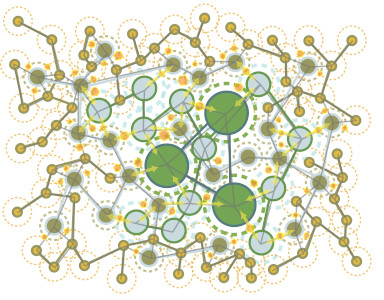
\includegraphics[height=0.25\textheight]{images/graph.jpg}\\
  \imageBased{Socialized Energy (AKA Smart Grid)}{Zachary Veach}{https://flic.kr/p/6rTacN}{CC BY-NC-SA 2.0}}

\usetikzlibrary{graphs}

\tikzset{defaultgraph/.style={>=stealth,every node/.style=graphnode,scale=#1}}

\newcommand{\samplegraph}[1][1.2]{%
  \begin{tikzpicture}[defaultgraph=#1]
    \node (1) at (1,2) {1};
    \node (2) at (3,2.2)   {2};
    \node (3) at (1.9,1.2)     {3};
    \node (4) at (0.8,0.3) {4};
    \node (5) at (2.5,0)   {5};
    \node (6) at (3.5,1.2) {6};
    \graph {
      (1) -> {(2), (3)};
      (2) -> (3);
      (3) -> {(4), (5)};
      (5) -> {(2), (4) ,(6)};
      (6) -> (2);
    };
  \end{tikzpicture}}

% изисквания към графа:
% да не е силно свързан (т.е. да има недостижим връх)
%% 1
% да има път, който се намира само след backtracking
%% 1 -> 2 -> 3 -> 4 <- 3 -> 5
% да има път, който минава през цикъл при първо минаване и пътят се намира едва след backtracking
%% 1 -> 2 -> 3 -> 5 -> 2 -> ... <- 5 -> 6
% да има път, който минава през цикъл, но в цикъла се влиза чак след backtracking, при първо минаване се намира пътя
%% 1 -> 2 -> 3 -> 4 <- 3 -> 5 -> 2 -> ...

\newcommand{\emptygraph}{%
\begin{tikzpicture}[defaultgraph=.8]
  \node (1) at (1,2)     {1};
  \node (2) at (3,2.2)   {2};
  \node (3) at (0.8,0.2) {3};
  \node (4) at (2.5,0)   {4};
\end{tikzpicture}}

\newcommand{\fullgraph}{%
\begin{tikzpicture}[defaultgraph=.8]
  \node (1) at (1,2)     {1};
  \node (2) at (3,2.2)   {2};
  \node (3) at (0.8,0.2) {3};
  \node (4) at (2.5,0)   {4};
  \graph {
    (1) -> {(2), (3), (4)};
    (2) -> {(1), (3), (4)};
    (3) -> {(1), (2), (4)};
    (4) -> {(1), (2), (3)};
  };
\end{tikzpicture}}

\begin{document}

\begin{frame}
  \titlepage
\end{frame}

\section{Дефиниции}

\begin{frame}
  \frametitle{Дефиниция на граф}
  \begin{definition}[Граф]
    (Ориентиран) граф е наредена двойка $(V,E)$, където
    \begin{itemize}
    \item $V \neq \emptyset$ е произволно множество от \textbf{върхове}
    \item $E \subseteq V^2$ е множество от наредени двойки върхове --- \textbf{ребра}
    \end{itemize}
  \end{definition}
  \pause
  Ако пренебрегнем реда на компонентите в двойките в $E$, получаваме \textbf{неориентиран} граф.\\[1em]
  \pause
  \begin{columns}[onlytextwidth]
    \begin{column}{0.5\textwidth}
      $E = \emptyset$ --- празен граф
      \emptygraph
    \end{column}
    \begin{column}{0.5\textwidth}
      $E = V^2$ --- пълен граф
      \fullgraph
    \end{column}
  \end{columns}
\end{frame}

\begin{frame}
  \frametitle{АТД: граф}
  Нелинейна структура, описваща обекти и връзките между тях.\\[1em]
  Операции:
  \begin{itemize}
  \item \tt{vertices()} --- списък на върховете
  \item \tt{successors(u)} --- списък на наследниците на даден връх
  \item \tt{isEdge(u, v)} --- проверка за съществуване на ребро
  \item \tt{addVertex(u)} --- включване на връх
  \item \tt{removeVertex(u)} --- изключване на връх
  \item \tt{addEdge(u, v)} --- включване на ребро
  \item \tt{removeEdge(u, v)} --- изключване на ребро
  \end{itemize}
\end{frame}

\begin{frame}
  \frametitle{Етикети}
  Обектите и връзките в графа могат да бъдат свързани с етикети.\\[1em]
  \pause
  Нека е дадено множество $L$ от етикети.
  \begin{itemize}
  \item $v : V \rightarrow L$ --- етикети на върховете
  \item $e : E \rightarrow L$ --- етикети на ребрата
  \end{itemize}
\end{frame}

\begin{frame}
  \frametitle{Допълнителни дефиниции}
  \begin{itemize}[<+->]
  \item за $(u, v)\in E$, $u$ наричаме \textbf{предшественик}, а $v$ --- \textbf{наследник}
  \item $(u, u)$ наричаме \textbf{примка}
  \item $d^+(u) = |\{ v\;|\;(u, v) \in E\}|$ --- \textbf{положителна полустепен}
  \item $d^-(v) = |\{ u\;|\;(u, v) \in E\}|$ --- \textbf{отрицателна полустепен}
  \item $d(u) = d^+(u) + d^-(u)$ --- \textbf{степен на връх}
  \item \textbf{път} в граф наричаме редица $v_1, v_2, \ldots, v_n$, където $(v_i, v_{i+1}) \in E$
    \begin{itemize}
    \item ако $v_1 = v_n$, пътят е \textbf{цикъл}
    \item ако $v_i \neq v_j$ за $1 \leq i < j \leq n$, пътят е \textbf{ацикличен}
    \item ако $E = \{(v_i,v_{i+1})\;|\;1 \leq i < j \leq n\}$ и $|E| = n - 1$, пътят е \textbf{Ойлеров}
    \item ако $V = \{v_i\;|\;1 \leq i \leq n\}$ и $|V| = n$, пътят е \textbf{Хамилтонов}
    \end{itemize}
  \item граф е \textbf{цикличен}, ако в него има поне един цикъл
  \item граф е \textbf{(слабо) свързан}, ако $\forall a, b\in V$ има път от $a$ до $b$ (или от $b$ до $a$)
  \end{itemize}
\end{frame}

\section{Предствания на графи}

\begin{frame}<1-19>
  \frametitle{Матрица на съседство}
  \footnotesize
  \begin{columns}[onlytextwidth]
    \begin{column}{0.5\textwidth}
      \begin{equation*}
        A =
        \left(
          \begin{array}{*6c}
            0 & 1 & 1 & 0 & 0 & 0\\
            0 & 0 & 1 & 0 & 0 & 0\\
            0 & 0 & 0 & 1 & 1 & 0\\
            0 & 0 & 0 & 0 & 0 & 0\\
            0 & 1 & 0 & 1 & 0 & 1\\
            0 & 1 & 0 & 0 & 0 & 0
          \end{array}
          \right)
      \end{equation*}
    \end{column}
    \begin{column}{0.5\textwidth}
      \samplegraph
    \end{column}
  \end{columns}
  \pause
  \vspace{-2ex}
  \begin{fixedarea}[.485]
    \alt<-14>{
      \begin{itemize}[<+->]
      \item $A_{i,j} = 1 \leftrightarrow (v_i,v_j) \in E$
      \item памет --- \rvl{$O(|V|^2)$}
      \item \tt{successors} --- \rvl{$O(|V|)$}
      \item \tt{isEdge} --- \rvl{$O(1)$}
      \item \tt{addVertex} --- \rvl{$O(|V|)$}
      \item \tt{removeVertex} --- \rvl{$O(|V|^2)$, ако се налага разместване}
      \item \tt{addEdge, removeEdge} --- \rvl{$O(1)$}
      \end{itemize}}{
      \begin{itemize}[<+(13)->]
      \item $A_{i,j} = 1 \leftrightarrow (v_i,v_j) \in E$
      \item $A^2_{i,j} > 0 \leftrightarrow \sum_{k=1}^n A_{i,k}A_{k,j} > 0 \leftrightarrow $ има път с дължина 2 от $v_i$ до $v_j$
      \item по индукция: $A^n_{i,j} > 0 \leftrightarrow $ има път с дължина $n$ от $v_i$ до $v_j$
      \item нещо повече: $A^n_{i,j}$ = броят на пътищата с дължина $n$ от $v_i$ до $v_j$
      \item ако $B = \sum_{k=1}^{|V|} A^k$, то $B_{i,j} > 0 \leftrightarrow$ има път от $v_i$ до $v_j$
      \end{itemize}}
  \end{fixedarea}
\end{frame}

\begin{frame}<1-12>[squeeze]
  \frametitle{Матрица на инцидентност}
  \begin{equation*}
    A =
    \left(
      \begin{array}{*9r}
         1 &  1 &  0 &  0 &  0 &  0 &  0 &  0 &  0\\
        -1 &  0 &  1 &  0 &  0 &  0 & -1 &  0 & -1\\
         0 & -1 & -1 &  1 &  1 &  0 &  0 &  0 &  0\\
         0 &  0 &  0 & -1 &  0 & -1 &  0 &  0 &  0\\
         0 &  0 &  0 &  0 & -1 &  1 &  1 &  1 &  0\\
         0 &  0 &  0 &  0 &  0 &  0 &  0 & -1 &  1
      \end{array}
    \right)
  \end{equation*}
  \vspace{-1.8ex}
  \begin{columns}[onlytextwidth]
    \begin{column}{0.7\textwidth}
      \begin{fixedarea}[.465]
        \alt<1>{%
          \begin{itemize}
          \item $A_{i,j} = 1 \leftrightarrow \exists v \in V\, e_j = (v_i, v) \leftrightarrow e_j\text{ е \textbf{изходящо} ребро за }v_i$
          \item $A_{i,j} = -1 \leftrightarrow \exists v \in V\, e_j = (v, v_i) \leftrightarrow e_j\text{ е \textbf{входящо} ребро за }v_i$
          \end{itemize}
        }{%
          \begin{itemize}[<+->]
          \item памет --- \rvl{$O(|V||E|)$}
          \item \tt{successors} --- \rvl{$O(|V||E|)$}
          \item \tt{isEdge} --- \rvl{$O(|E|)$}
          \item \tt{addVertex} --- \rvl{$O(|E|)$}
          \item \tt{addEdge} --- \rvl{$O(|V|)$}
          \item \tt{removeVertex, removeEdge} --- \rvl{$O(|V||E|)$, ако се налага разместване}
          \end{itemize}
        }
      \end{fixedarea}
    \end{column}
    \begin{column}{0.3\textwidth}
      \samplegraph[1]
    \end{column}
  \end{columns}
\end{frame}

\begin{frame}
  \frametitle{Списък на наследници}
  \footnotesize
  \begin{columns}[onlytextwidth]
    \begin{column}{0.5\textwidth}
      \begin{equation*}
      D = \left\{
      \begin{array}{rcl}
        1 &\rightarrow& (2, 3)\\
        2 &\rightarrow& (3)\\
        3 &\rightarrow& (4, 5)\\
        4 &\rightarrow& ()\\
        5 &\rightarrow& (2, 4, 6)\\
        6 &\rightarrow& (2)
      \end{array}\right\}
  \end{equation*}
    \end{column}
    \begin{column}{0.5\textwidth}
      \samplegraph[1]
    \end{column}
  \end{columns}
  \vspace{-2ex}
  \begin{fixedarea}[.55]
    \begin{itemize}[<+->]
    \item $D_i = \{v\;|\;(v_i,v) \in E \}$, може да е множество или списък
    \item памет --- \rvl{$O(|V|+|E|)$}
    \item \tt{successors} --- \rvl{$O(1)$}
    \item \tt{isEdge} --- \rvl{$O(|V|)$ (ако е множество --- $O(1)$)}
    \item \tt{addVertex} --- \rvl{$O(1)$}
    \item \tt{removeVertex} --- \rvl{$O(|E|)$, трябва да се премахнат входящите ребра}
    \item \tt{addEdge} --- \rvl{$O(1)$}
    \item \tt{removeEdge} --- \rvl{$O(|V|)$ (ако е множество --- $O(1)$)}
    \end{itemize}
  \end{fixedarea}
\end{frame}

\begin{frame}
  \frametitle{Списък на инцидентност}
  \begin{columns}[onlytextwidth]
    \begin{column}{0.5\textwidth}
      \begin{equation*}
        \begin{array}{rll}
          E = ((1,2),&(2,3),&(5,6),\\
          (1,3),&(3,5),&(3,4),\\
          (5,2),&(5,4),&(6,2))
        \end{array}
      \end{equation*}
    \end{column}
    \begin{column}{0.5\textwidth}
      \samplegraph[1]
    \end{column}
  \end{columns}
  \vspace{-.5ex}
  \begin{fixedarea}[.51]
    \begin{itemize}[<+->]
    \item може да е представено като списък или множество
    \item памет --- \rvl{$O(|E|)$}
    \item \tt{successors} --- \rvl{$O(|E|)$}
    \item \tt{isEdge} --- \rvl{$O(|E|)$ (ако е множество --- $O(1)$)}
    \item \tt{addVertex, addEdge} --- \rvl{$O(1)$}
    \item \tt{removeVertex} --- \rvl{$O(|E|)$}
    \item \tt{removeEdge} --- \rvl{$O(|E|)$ (ако е множество --- $O(1)$)}
    \end{itemize}
  \end{fixedarea}
\end{frame}

\begin{frame}
  \frametitle{Локални задачи}
  \textbf{Задача. }Да се намерят върховете, които нямат наследници.\\
  \pause
  \textbf{Решение. }$\{u\;|\;\nexists v\, (u,v) \in E\}$\\[1em]
  \pause
  \textbf{Задача. }Да се намерят предшествениците на даден връх $v$.\\
  \pause
  \textbf{Решение. }$\{u\;|\;(u,v)\in E\}$\\[1em]
  \pause
  \textbf{Задача. }Да се провери дали граф е симетричен.\\
  \pause
  \textbf{Решение. }$\forall u,v\in V[(u,v)\in E \rightarrow (v,u)\in E]$
\end{frame}

\section{Схеми за обхождане}

\begin{frame}
  \frametitle{Обхождане в дълбочина}
  \begin{columns}[T,onlytextwidth]
    \begin{column}{0.6\textwidth}
      \begin{block}{}
        Обхождане на връх \tt v:
        \begin{itemize}
        \item Обходи последователно всички наследници на \tt v
        \end{itemize}
      \end{block}
    \end{column}
    \begin{column}{0.1\textwidth}
    \end{column}
    % TODO: анимация с TikZ
    \begin{column}{0.3\textwidth}
      \samplegraph[1]
    \end{column}
  \end{columns}
  \pause
  \vspace{-6ex}
  \begin{itemize}[<+->]
  \item \alert{Имаме ли дъно?}
    \begin{itemize}
    \item Да: при празен списък от наследници!
    \end{itemize}
  \item \alert{Какво се случва ако графът е цикличен?}
    \begin{itemize}
    \item Програмата също зацикля! Как да се справим с този проблем?
    \item Трябва да помним през кои върхове сме минали!
    \end{itemize}
  \end{itemize}
  \begin{enumerate}[<+->]
  \item да помним текущия път
    \begin{itemize}
    \item<9-> намираме всички ациклични пътища
    \item<10-> сложност $O(|V||V|!)$
    \end{itemize}
  \item да помним всички обходени до момента върхове
    \begin{itemize}
    \item<9-> обхождаме всеки връх по един път
    \item<10-> сложност $O(|E|)$
    \end{itemize}
  \end{enumerate}
\end{frame}

\begin{frame}[squeeze]
  \frametitle{Схема на обхождане в ширина}

  \begin{columns}[T,onlytextwidth]
    \begin{column}{0.6\textwidth}
      \vspace{-3ex}
      \begin{block}{}
        Обхождане, започващо от връх \tt u:
        \vspace{-.5ex}
        \begin{itemize}
        \item Маркира се \tt u за обхождане на ниво 1
        \item За всеки връх \tt v маркиран за ниво $n$:
          \begin{itemize}
          \item Маркират се всички наследници \tt s на \tt v за обхождане на
            ниво $n+1$
          \end{itemize}
        \end{itemize}
      \end{block}
    \end{column}
    \begin{column}{0.1\textwidth}
    \end{column}
    % TODO: анимация с TikZ
    \begin{column}{0.3\textwidth}
      \samplegraph[1]
    \end{column}
  \end{columns}
  \vspace{-3ex}
  \onslide<+->
  \begin{itemize}[<+->]
  \item \alert{Какво се случва ако графът е цикличен?}
    \begin{itemize}
    \item Ако има път: намира го.
    \item Ако няма път: програмата зацикля!
    \item Трябва да помним през кои върхове сме минали!
    \end{itemize}
  \end{itemize}
  \begin{enumerate}[<+->]
  \item да помним текущия път за всеки връх в текущото ниво
    \begin{itemize}
    \item<8-> обхождаме с повторение на върховете (всички ациклични пътища)
    \item<9-> сложност по време \textbf{и памет} $O(|V||V|!)$
    \end{itemize}
  \item да помним всички обходени до момента върхове
    \begin{itemize}
    \item<8-> обхождаме всеки връх по един път
    \item<9-> сложност $O(|E|)$ по време и $O(|V|)$ по памет
    \end{itemize}
  \end{enumerate}
\end{frame}

\begin{frame}
  \frametitle{Сравнение на обхождане в дълбочина и ширина}
  Обхождането в дълбочина\ldots
  \pause
  \begin{itemize}[<+->]
  \item \ldots използва памет само за обходените до момента върхове
  \item \ldots е подходящо за задачи, където търсим единична цел, която е „надълбоко“
  \item \ldots може да обхожда избрани пътища преференциално
  \item \ldots естествено се реализира с \textbf{рекурсия}
  \end{itemize}
  \onslide<+->
  Обхождането в ширина\ldots
  \begin{itemize}[<+->]
  \item \ldots използва памет за всички разглеждани нива
  \item \ldots е подходящо за задачи, където търсим „най-плитката“ цел
  \item \ldots обхожда графа „равномерно“
  \item \ldots естествено се реализира с \textbf{итерация}
  \end{itemize}
\end{frame}

\section{Задачи с обхождане}

\begin{frame}
  \frametitle{Търсене на път}
  \textbf{Задача. } Да се намери път между върховете $u$ и $v$, ако такъв има.\\\pause
  Търсене на път \textbf{в дълбочина}
  \pause
  \begin{itemize}[<+->]
  \item удобно е да пазим текущия път в \textbf{стек}
  \item при стъпка напред (последване на наследник) добавяме в стека
  \item при стъпка назад (няма повече наследници) махаме от стека
  \item има път от $u$ до $v$, ако:
    \begin{itemize}
    \item $u = v$ (дъно)
    \item $\exists w\, (u,w)\in E\;\&\;$има път от $w$ до $v$
    \end{itemize}
  \end{itemize}
  \onslide<+->
  Търсене на път \textbf{в ширина}
  \begin{itemize}[<+->]
  \item удобно е да пазим в \textbf{стек} обходените \textbf{ребра}
  \item винаги намираме най-късия по брой ребра път
  \item конструираме пътя като се връщаме назад по ребрата
  \item има път от $u$ до $v$, ако при обхождане, стартиращо от $u$, съществува  ниво $n$, така че на него обхождаме $v$
  \end{itemize}
\end{frame}

\begin{frame}
  \frametitle{Намиране на всички пътища}
  \textbf{Задача. } Да се намерят всички пътища, започващи от върха $u$.\pause
  \begin{itemize}[<+->]
  \item ако графът е цикличен, пътищата са безкрайно много!
  \item можем да търсим всички \textbf{ациклични} пътища
  \item трябва да изследваме всички възможни комбинации от ребра\ldots
  \item \ldots което означава, че трябва да позволим повтарянето на върхове!
  \item търсене в \textbf{дълбочина}
    \begin{itemize}
    \item при стъпка назад макрираме върха като непосетен
    \item всъщност посетените върхове са точно тези от текущия път!
    \end{itemize}
  \item търсене в \textbf{ширина}
    \begin{itemize}
    \item ако в нивото пазим само ребрата: връщайки се назад трябва да изпробваме рекурсивно всички възможни комбинации
      \begin{itemize}
      \item става еквивалентно на търсене в дълбочина!
      \end{itemize}
    \item ако в нивото пазим целия път: при завършване на обхождането получаваме списък от всички ациклични пътища
    \item компромисен вариант: вместо път пазим връх и указател към предшественик
      \begin{itemize}
      \item не намалява сложността по памет в най-лошия случай!
      \end{itemize}
    \end{itemize}
  \end{itemize}
\end{frame}

\begin{frame}
  \frametitle{Намиране на цикли}
  \textbf{Задача. }Да се намери цикъл в даден граф, ако такъв има.\\
  \pause
  \textbf{Решение:}\\
  \begin{itemize}[<+->]
  \item започваме от произволен връх $u$
  \item обхождаме в ширина или дълбочина
  \item запомняме обходените върхове и не ги обхождаме повторно
  \item запомняме пътя (както при търсене на път)
  \item ако достигнем вече обходен връх --- има цикъл, връщаме намерения път
  \item ако успеем да обходим всички ребра --- няма цикъл
  \end{itemize}
\end{frame}

\begin{frame}
  \frametitle{Покриващо дърво}
  \begin{definition}
    \small
    \textbf{Дърво} наричаме ацикличен граф, в който има единствен връх $r$, така че:
    \begin{itemize}
    \item $r$ няма предшественици ($d^-(r) = 0$)
    \item другите върхове имат точно един предшественик ($\forall v\neq r\;d^-(v) = 1$)
    \end{itemize}
  \end{definition}
  \pause
  \textbf{Задача. }По даден (свързан) граф $(V,E)$ да се намери дърво $(V,E')$ за $E' \subseteq E$.\\
  \pause
  \textbf{Решение:}\\
  \begin{itemize}[<+->]
  \item обхождаме в дълбочина или ширина
  \item запомняме обходените върхове и не ги обхождаме повторно
  \item добавяме в дървото всеки нов връх и реброто, по което сме дошли до него
  \item приключваме при обхождане на всички върхове
  \end{itemize}
\end{frame}

\begin{frame}
  \frametitle{Топологично сортиране}
  \textbf{Задача. }По даден граф $(V,E)$ търсим пермутация на върховете $v_{i_1},v_{i_2},\ldots,v_{i_n}$, така че $\forall (u,w)\in E\,\exists j < k\,(u = v_{i_j}\,\&\,w = v_{i_k})$.\\
  \pause
  \textbf{Решение: }Събираме списък от върхове $l$\\
  \begin{itemize}[<+->]
  \item първоначално в $l$ поставяме всички $u\in V$, за които $d^-(u) = 0$
  \item обхождаме $l$ от началото, като за всеки обходен връх $u$:
    \begin{itemize}
    \item за всеки наследник $v$ на $u$
      \begin{itemize}
      \item премахваме реброто $(u,v)$ от графа
      \item ако $d^-(v) = 0$ добавяме го в края на $l$
      \end{itemize}
    \end{itemize}
  \item ако изчерпим $l$, но в графа останат още ребра --- грешка, имало е цикъл
  \item в противен случай, $l$ е решение на задачата
  \end{itemize}
\end{frame}

\end{document}
